\chapter{Implémentation}
\section{Structures de données}
\paragraph{}
La stratégie de recherche avec graphe requiert une représentation des entrées du problème, des états construisant une solution potentielle à ce dernier ainsi que le développement de ces états.
\subsection{Représentation du problème SAT}
\paragraph{}
Une instance du problème SAT peut être considérée comme un ensemble de clauses, chacune de ces clauses est une disjonction de littéraux. Dans ce rapport Nous proposons deux structures différentes pour les représenter que nous comparerons par la suite.
\subsubsection{Représentation matricielle}
\paragraph{}
Une première représentation serait d‘associer à chaque clause de l’instance un tableau de taille égale au nombre de variables logiques utilisés dont la i\up{ième}  case aura la valeur 1 si la variable \textit{i} est présente dans la clause, -1 si sa négation est présente, 0 sinon. Ainsi en représentant toutes les clauses on obtient une matrice dont chaque ligne est associée à une clause.\\
L’exemple suivant montre une instance du problème SAT et sa représentation matricielle:
\begin{flalign*}
x_{1} \lor \neg x_{2} \lor x_{5} \\
\neg x_{2} \lor x_{4} \lor x_{5} \\
\neg x_{1} \lor x_{2} \lor \neg x_{3}
\end{flalign*}
Ces clauses vont être représentée comme suit:
\begin{center}
	\parbox{.2\textwidth}{
		\begin{tabular}{|c|c|c|c|c|}
			\hline
			1&-1&0&0&1\\
			\hline
			0&-1&0&1&1\\
			\hline
			-1&1&1&0&0\\
			\hline
		\end{tabular}}
\end{center}
\newpage

\subsubsection{Représentation par \textit{Bitset}}
\paragraph{}
On pourrait aussi aborder la représentation du point de vu littéral, c’est à dire associer à chaque littéral les clauses dans lesquels il est présent. Pour cela un tableau de bits appelé \textit{Bitset} pourrait être utilisé où chaque bit \textit{i} aurait la valeur 1 si la i\up{ième} clause contient le littéral, la valeur 0 sinon. On obtient donc un tableau de taille 2 fois le nombre de variables utilisés dont les entrés représentent les \textit{Bitsets} des littéraux.\\
Pour le même exemple vu précédemment on obtient les \textit{Bitsets} suivants:\\\\
	\begin{minipage}{0.5\textwidth}
		\centering
		\begin{tabular}{|c | c| c| c|}
			\hline
			$x_{1}$& 1 & 0 & 0 \\\hline
			$x_{2}$& 0 & 0 & 0 \\\hline
			$x_{3}$& 0 & 0 & 0 \\\hline
			$x_{4}$& 0 & 1 & 0 \\\hline
			$x_{5}$& 1 & 1 & 0 \\\hline
		\end{tabular}
	\end{minipage}
	\hfillx
	\begin{minipage}{0.5\textwidth}
		\centering
		\begin{tabular}{|c | c| c| c|}
			\hline
			$\neg x_{1}$& 0 & 0 & 1 \\\hline
			$\neg x_{2}$& 1 & 1 & 0 \\\hline
			$\neg x_{3}$& 0 & 0 & 1 \\\hline
			$\neg x_{4}$& 0 & 0 & 0 \\\hline
			$\neg x_{5}$& 0 & 0 & 0 \\\hline
		\end{tabular}
	\end{minipage}

\subsection{Représentation des états}
\paragraph{}
Une solution à une instance du problème SAT se réduit à l’assignation des valeurs de vérités aux variables logiques de cette instance. On peut considérer un état dans l’espace de recherche comme étant le choix de la valeur de vérité d’une des variables logiques, on obtient après une succession de choix une solution au problème qui peut être positive si les valeurs assignés sont consistante avec les clauses de l’instance, négative sinon. Nous allons représenter un état avec un noeud qui contient le numéro de la variable choisie, multiplié par -1 pour désigner l’assignation de la valeur $faux$ à la variable, il reste inchangé sinon.\\
\begin{center}
	\begin{forest} [
		[5[$x_{5} \leftarrow vrai$]]
		[-5[$x_{5} \leftarrow faux$]]
		]
	\end{forest}
\end{center}
\newpage
\subsection{Développement des états}
\paragraph{}
A partir de chaque état on peut faire le choix de la valeur de vérité d’une variable logique choisie aléatoirement. Le développement d’un noeud donne deux successeurs, un pour chaque valeur de vérité assignée à la prochaine variable. On obtient après l’exploration de l’espace de recherche un arbre d’états, l’exemple suivant est un arbre associé à une instance SAT contenant trois variables.\\
\begin{center}
	\begin{forest} [
		[2
			[1
				[3]
				[-3]
			]
			[-1
				[3]
				[-3]
			]
		]
		[-2
			[1
				[3]
				[-3]
			]
			[-1
				[3]
				[-3]
			]
		]
		]
	\end{forest}
\end{center}
Une solution est représentée par une branche de l’arbre, par exemple la solution : $x_{1} = vrai$, $x_{2} = faux$, $x_{3} = faux$ est représentée dans l’arbre précédent comme suit:
\begin{center}
	\begin{forest} [
		[2
		[1
		[3]
		[-3]
		]
		[-1
		[3]
		[-3]
		]
		]
		[-2, text=red
		[1, text=red
		[3]
		[-3, text=red]
		]
		[-1
		[3]
		[-3]
		]
		]
		]
	\end{forest}
\end{center}
Pour pouvoir construire une solution à partir de n’importe quel noeud, on doit y sauvegarder l’adresse de son parent, ainsi on peut récupérer les valeurs assignées aux noeuds précédents jusqu’à la racine. L’enregistrement suivant représente un noeud de l’arbre:

\begin{lstlisting}
struct {
int valeur; 
struct noeud* parent;
} noeud;
\end{lstlisting}

\paragraph{Remarque1:}\label{BreadthIssue} Un inconvénient que nous avons déjà cité de la recherche en largeur d’abord était la saturation rapide de la mémoire, cela est dû au fait de garder tous les noeuds dans la mémoire. Ce problème est évité dans la recherche en profondeur d’abord car dès l’évaluation d’un noeud se trouvant dans la profondeur maximale, ce dernier est supprimé de la mémoire. notons que la structure du noeud déjà présenté ne contient pas les adresses de ses successeurs, ceci nous permet d’éviter de garder tous l’arbre d’états dans la mémoire mais juste les branche susceptible d’être évaluée par la suite.\\~\\
\paragraph{Remarque2:} Dans la deuxième représentation du problème SAT, une optimisation serait d’ajouter un $Bitset$ dans la structure du noeud et y garder les clauses qu’il satisfait ainsi que celles de ses parents, celui là peut être obtenu en appliquant l’opération OU logique sur le $Bitset$ du noeud parent et celui du littéral choisi.\\
\begin{center}
	\begin{minipage}{0.5\textwidth}
		\centering
		\begin{tabular}{|c | c| c| c|c|}
			\hline
			$Bitset$ du parent& 1 & 0 & 1 & 1 \\\hline
		\end{tabular}
	\end{minipage}
	\\~\\
	OR
	\\~\\
	\begin{minipage}{0.5\textwidth}
		\centering
		\begin{tabular}{|c | c| c| c|c|}
			\hline
			$Bitset$ du littéral& 1 & 0 & 0 & 1\\\hline
		\end{tabular}
	\end{minipage}
	\begin{center}

		$\downarrow$
		\\~\\
		\begin{tabular}{|c | c| c| c|c|}
			\hline
			$Bitset$ du noeud& 1 & 0 & 1 & 1\\\hline
		\end{tabular}
	\end{center}
\end{center}

\section{Conception et pseudo-code}
\paragraph{}
Dans cette partie nous allons présenter l’implémentation des algorithmes de recherche avec graphe, un algorithme générique qui englobe les différente méthodes est présenté si dessous:

\begin{algorithm}
	\SetAlgoLined
	\KwResult{retourne la solution ou échec}
	$open \gets \textbf{état initial}$\;
	initialiser l'ensemble $closed$ à \textbf{vide}\;
	\While{$\neg$\textbf{vide} $open$}{
		$noeud \gets$ \textbf{choisir\_noeud($open$)}\;
		\If{\textbf{noeud\_but}($noeud$)}{
			\Return \textbf{solution}($noeud$)\;
		}
		\textbf{ajouter}($noeud$,$closed$)\;
		$successeurs \gets$ \textbf{developper}($noeud$) \;
		inserer les $sueccesseurs$ qui n'appartiennent pas à $closed$ dans $open$ 
	}
	\Return echec\;
\caption{Algorithme de recherche avec graphe}
\end{algorithm}
\paragraph{}
La différence entre les algorithmes de recherche réside dans la manière dont on sélectionne le noeud à évaluer, ligne 4 dans l’algorithme si dessus, ainsi que l’estimation du coût et de l’heuristique, s’ils existent, avant l’insertion, ligne 10.\\
\paragraph{}
En se basant sur cette algorithme nous avons implémenter une procédure de recherche générique prenant en paramètre un type de gestion de liste, un estimateur de coût et d’heuristique et les entrés de l’instance SAT afin d’évaluer les noeuds.
\subsection{Gestion de la liste open}
\paragraph{}

\subsubsection{Profondeur d'abord}
La recherche en profondeur d’abord consiste à choisir le noeud avec la profondeur la plus élevé de l’arbre, ceci reviens à sélectionner l’élément le plus récemment inséré dans la liste open, c’est à dire, la gérer avec une politique LIFO.\\
Insertion d'un noeud:\\
\begin{minipage}{0.5\textwidth}
	\centering
	\begin{tabular}{|c |}
		\hline
		 3 \\
		\hline
	\end{tabular}
\end{minipage}
\hfillx
$\rightarrow$
\begin{minipage}{0.5\textwidth}
	\centering
	\begin{tabular}{|c | c| c| c|}
		\hline
		{\color{red}3} & -3 & -2 & -1 \\\hline
	\end{tabular}
\end{minipage}

Sélection d'un noeud:\\
\begin{minipage}{0.5\textwidth}
	\centering
	\begin{tabular}{|c |}
		\hline
		{\color{red}3} \\
		\hline
	\end{tabular}
\end{minipage}
\hfillx
$\leftarrow$
\begin{minipage}{0.5\textwidth}
	\centering
	\begin{tabular}{| c| c| c|}
		\hline
		-3 & -2 & -1 \\\hline
	\end{tabular}
\end{minipage}


\subsubsection{Largeur d'abord}
\paragraph{}

Contrairement à la recherche en profondeur d’abord, les noeuds sont visités de tel sorte à parcourir l’arbre niveau par niveau, cela peut être réalisé par la sélection du noeud le moins récemment insérer dans open, d’où une gestion LIFO de la liste.\\
Insertion d'un noeud:\\
\begin{minipage}{0.5\textwidth}
	\centering
	\begin{tabular}{|c |}
		\hline
		3 \\
		\hline
	\end{tabular}
\end{minipage}
\hfillx
$\rightarrow$
\begin{minipage}{0.5\textwidth}
	\centering
	\begin{tabular}{|c | c| c| c|}
		\hline
		{\color{red}3} & -3 & -2 & -1 \\\hline
	\end{tabular}
\end{minipage}

Sélection d'un noeud:\\
\begin{minipage}{0.5\textwidth}
	\centering
	\begin{tabular}{|c |}
		\hline
		{\color{red}-1} \\
		\hline
	\end{tabular}
\end{minipage}
\hfillx
$\leftarrow$
\begin{minipage}{0.5\textwidth}
	\centering
	\begin{tabular}{| c| c| c|}
		\hline
		3 & -3 & -2  \\\hline
	\end{tabular}
\end{minipage}

\subsubsection{Recherche En se basant sur une fonction d'évaluation}
\paragraph{}
Dans ce type de recherche, la sélection d’un noeud se fait sur la base d’une fonction d’évaluation. Le noeud sélectionné est celui avec la valeur minimale (resp. maximale) de la fonction d’évaluation. Nous utilisons ce type de gestion afin d’implémenter les algorithmes: recherche à coût uniforme, recherche gloutonne et l’algorithme A*.\\
Nous avons implémenter ce type de gestion avec deux structures différentes que nous comparerons dans la suite de ce rapport.
\paragraph{Liste triée}
Les noeuds sont triés dans une liste selon leur valeur estimé par la fonction d’évaluation. Le premier noeud est toujours sélectionner, l’insertion par contre se fait de tel sorte à garder la liste triée en ordre croissant (resp. décroissant).\\
Insertion d'un noeud:\\
\begin{minipage}{0.5\textwidth}
	\centering
	\begin{tabular}{|c |c|}
		\hline
		3 & $f_{3}=5$\\
		\hline
	\end{tabular}
\end{minipage}
\hfillx
$\rightarrow$
\begin{minipage}{0.5\textwidth}
	\centering
	\begin{tabular}{| c| c|c | c| c| c|}
		\hline
		 -3& $f_{-3}=2$ & {\color{red}3}& {\color{red}$f_{3}=5$} & -1& $f_{-1}=8$ \\\hline
	\end{tabular}
\end{minipage}

Sélection d'un noeud:\\
\begin{minipage}{0.5\textwidth}
	\centering
	\begin{tabular}{|c |c|}
		\hline
		{\color{red}-3} & {\color{red}$f_{-3}=2$}\\
		\hline
	\end{tabular}
\end{minipage}
\hfillx
$\leftarrow$
\begin{minipage}{0.5\textwidth}
	\centering
	\begin{tabular}{|c | c| c| c|}
		\hline
		3& $f_{3}=5$ & -1& $f_{-1}=8$ \\\hline
	\end{tabular}
\end{minipage}\\~\\
Complexité de l’insertion : $o(n)$.\\
Complexité de la sélection : $o(1)$.\\


\paragraph{Tas}
Les noeuds sont organisé dans une structure de tas\footnote{un tas est un arbre équilibré dont chaque noeud a une clé supérieur (resp. Inférieur) à celle de ses fils}. La racine du tas est sélectionner pour l’évaluation, tandis que l’insertion se fait par entassement du nouveau élément. Les deux opérations se font en $o(log(n))$.

\subsection{Fonction d'évaluation}
\paragraph{}
La fonction d’évaluation f d’un noeud n est généralement définit à l’aide de deux autres fonctions g et h. La première désigne le coût nécessaire pour atteindre le noeud n à partir de la racine, tandis que la deuxième est une heuristique qui estime le coût restant avant d’arriver au but.
\subsubsection{Recherche gloutonne}
\paragraph{}
La fonction d’évaluation dans ce cas f est égale à h, on se contente de la valeur estimé par l’heuristique pour décider le prochain noeud à développer. Une heuristique pour le problème SAT qui peut mesurer la distance des noeuds par rapport au noeud but serait de calculer le nombre de clauses pas encore satisfaites, le noeud avec la valeur minimale de cette heuristique est le noeud qui satisfait le plus de clauses et donc le plus proche de satisfaire toutes les clauses.
\subsubsection{Recherche à coût uniforme}
\paragraph{}
Contrairement à la recherche gloutonne, la recherche à coût uniforme n’utilise que la fonction g, permettant ainsi de développer le noeud le plus proche de la racine en terme de coût. Cependant trouver une fonction d’estimation du coût pour le problème SAT s’avère délicat comme on ne peut pas vraiment déterminer une distance entre un noeud et la racine. Ceci dit, une fonction de coût qui calcule le nombre de clauses devant être satisfaite par un noeud mais qui sont déjà satisfaite par ses parents peut être utilisé. Cela représente la perte d’une branche contenant des littéraux qui satisfont les même clauses de l’instance SAT, plus le coût est élevé, moins les chances que cette branche nous mène au but.
\newpage
\begin{minipage}{0.5\textwidth}
	\centering
	\begin{tabular}{|c | c| c| c|c|}
		\hline
		$Bitset$ du parent& {\color{red}1} & 0 & 0 & 1 \\\hline
	\end{tabular}
\end{minipage}
$\rightarrow$
\begin{minipage}{0.5\textwidth}
	\centering
	\begin{tabular}{|c | c| c| c|c|}
		\hline
		$Bitset$ du littéral& {\color{red}1} & 1 & 0 & 0\\\hline
	\end{tabular}
\end{minipage}
\begin{center}
	coût = 1
\end{center}

\subsubsection{Algorithme A*}
\paragraph{}
L’algorithme A* combine les deux fonctions g et h citées précédemment afin d’évaluer les noeuds en prenant en considération le nombre de clauses déjà satisfaites ainsi que le coût de la branche dans laquelle il se trouve.
\subsection{Évaluateur SAT}
\paragraph{}
Dans cette partie nous présentons deux méthodes d’évaluation du noeud but basé sur les deux structures représentatives des instances SAT citées précédemment.
\subsubsection{Évaluation par matrice}
\paragraph{}\label{def:matrix}
La première méthode consiste à parcourir la matrice des clauses et chercher pour chaque clause si un de ses littéraux a été évalué vrai par les noeuds de la solution. Si dessous l’algorithme correspondant.\\
\begin{algorithm}
	\SetAlgoLined
	\KwResult{retourne un booléen: vrai si la solution est positive, faux sinon}
	\textbf{entré}: $solution$\;
	\For{$clause \in$ $matrice$}{
		$satC\gets faux$ \;
		\For{$noeud \in$ $solution$ et $\neg satC$}{
			\If{$clause[\textbf{abs}(noeud.valeur)]\times$ $noeud.valeur$ > 0}
			{
				$satC\gets vrai$\;
			}
		}
		\If{$satC$}{
			$cpt \gets$ $cpt + 1$\;	
		}
		
	}
	\If{$cpt = \textbf{taille}(matrice)$}
	{
		\Return $vrai$\;
	}
	\Return $faux$\;
	\caption{Algorithme d'évaluation par matrice}
\end{algorithm}
\subsubsection{Évaluation par Bitset}
\paragraph{}\label{def:Bitset}
Comme vu précédemment, en utilisant la structure Bitset pour représenter l’instance SAT chaque noeud contient un Bitset des clauses satisfaites par sa branche, il suffit donc de calculer le nombre de bits à 1 pour décider si c’est un noeud but ou pas. Nous utilisons pour cela l’algorithme “Hamming Weight” permettant de calculer le nombre de bits à 1 dans un entier en une complexité constante.
\section{Interface graphique}
\paragraph{}
Afin de faciliter l'utilisation des méthodes, et la visualisation en temps réel du comportemment de ces dernière, nous avons mis au point une interface graphique simple d'utilisation.
\paragraph{}
La fenêtre principale se décompose en quatres sections ( voir figure ci dessous \ref{fig:mainWindow} )
\begin{figure}[H]
	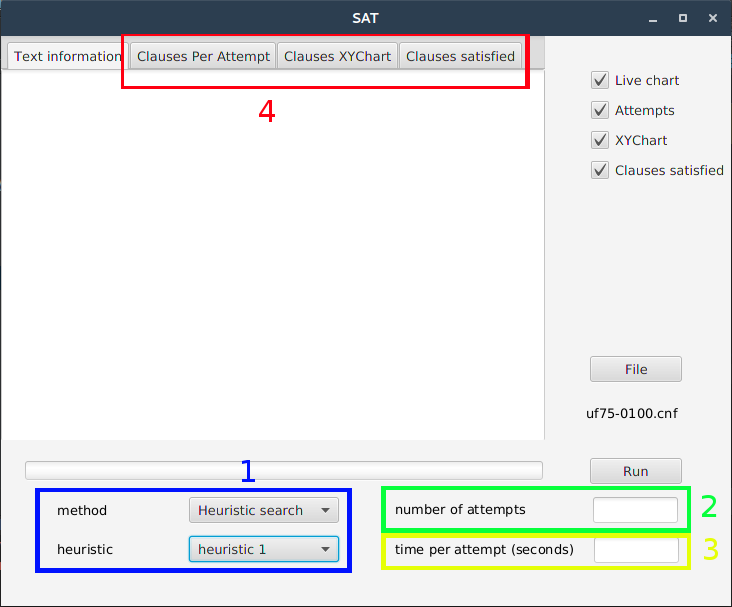
\includegraphics[width=\textwidth]{images/imgs/interface.png}
	\label{fig:mainWindow}
	\caption{Fenêtre principale }
\end{figure}
\newpage
\paragraph{Détails}
\begin{enumerate}
	\item Une liste déroulante pour choisir la méthode de recherche désirée.
	\item Le nombre de tentatives sur une même instance.
	\item La durée (en secondes) d'une tentative sur une instance.
	\item Un groupe d'onglets dédiés à l'affichage de trois types de graphiques illustratifs.
\end{enumerate}
\paragraph{}
Pour ce qu'il en est des groupes d'onglets, nous avons trois types de graphiques : 
\begin{itemize}
	\item \textbf{Attempts : } un histogramme montrant le taux de satisfiabilité pour chaque tentatives sur une instances : 
	\begin{figure}[H]\label{attemptsChart}
		\centering
		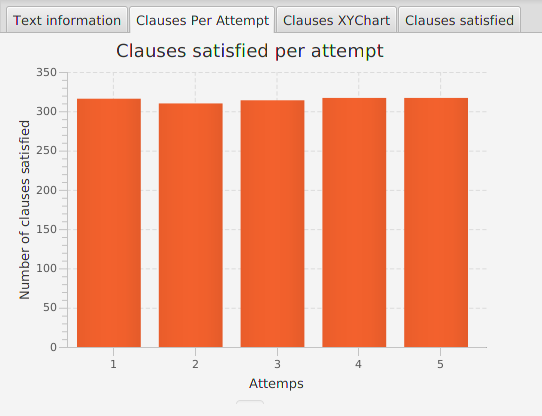
\includegraphics[scale=0.5]{images/imgs/attemptsChart.png}
		\caption{Attempts}
	\end{figure}
	\item \textbf{XYChart : } une courbe pour suivre l'évolution du taux de satisfiabilité pour chaque tentative : 
	\begin{figure}[H]\label{XYchart}
		\centering
		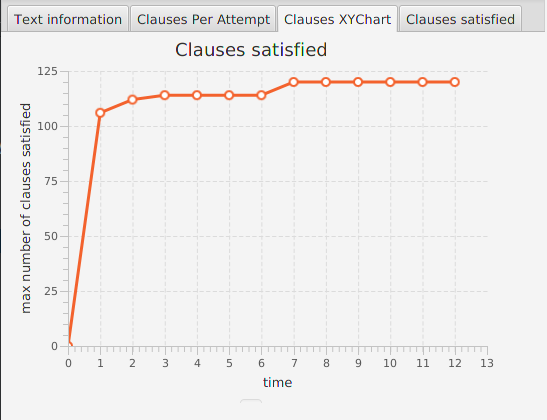
\includegraphics[scale=0.5]{images/imgs/XYChart.png}
		\caption{XYChart}
	\end{figure}
	\item \textbf{Clauses satisfied : } un histogramme qui montre la fréquence de satisfiabilité d'une clause $c_i$ durant une tentative sur l'instance courante, l'histogramme est trié pour mieux observer les données : 
	\begin{figure}[H]\label{frequencies}
		\centering
		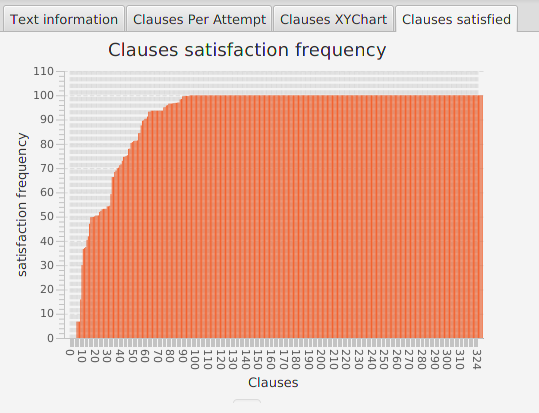
\includegraphics[scale=0.5]{images/imgs/frequenciesChart.png}
		\caption{Clauses satisfied }
	\end{figure}
\end{itemize}